\chapter{Objetivos}\label{cap.Objetivos}
\hspace{1 cm} Una vez presentado el contexto de este TFG en el primer cap\'itulo, tanto en general como el m\'as cercano, en este cap\'itulo se van a explicar los objetivos concretos a conseguir y la metodolog\'ia utilizada para llegar a ello.

\section{Objetivo principal}
\hspace{1 cm} El objetivo propuesto de este trabajo es conseguir que un drone navegue desde una baliza de partida a otra baliza de llegada, que debe reconocerse por visi\'on y cuya posici\'on es desconocida. Para esto, se han propuesto tres fases principales:

\begin{itemize}
\item \textbf{Percepci\'on visual:} La percepci\'on se basa un filtro de color. Dada una imagen de entrada, se deber\'a detectar una baliza previamente asignada para, en funci\'on de lo obtenido, enviar una informaci\'on u otra al drone. Habr\'a que tener en cuenta objetos que sean del mismo color de la baliza, los cuales querremos descartar para que no interfieran. 

\item \textbf{Control:} En funci\'on de lo que perciba y del momento en el que se encuentre, se tomar\'a una u otra decisi\'on para realizar los movimientos oportunos en cada momento. Es importante que \'estos no sean bruscos, provocando desestabilizaciones del drone.

\item \textbf{Validaci\'on experimental:} Cada vez que se da un avance en los apartados anteriores, hay que validar su funcionamiento, tanto en simulaci\'on como en el drone

\end{itemize}

\section{Requisitos}
\hspace{1 cm} Para la realizaci\'on de los objetivos anteriormente citados, se tiene que conseguir una soluci\'on que cumpla las siguientes caracter\'isticas:
\begin{itemize}
\item  Que funcione sobre JdeRobot-5.4.2, utilizando las herramientas necesarias para el control del drone, filtros de color y diagrama de estados. 
\item  Que el algoritmo sea vivaz, la frecuencia de iteraciones es importante para un comportamiento \'agil y fluido del drone, el procesamiento de im\'agenes o el control del drone no puede ser pesado computacionalmente, pues puede llevar a un algoritmo lento, y por lo tanto un mal control del drone. 
\item  Que el algoritmo sea robusto, teniendo que funcionar tanto en el simulador, con im\'agenes puras y sin perturbaciones del vuelo, como en el drone real ArDrone2 de Parrot, donde las im\'agenes no son ideales, existe ruido o donde s\'i hay corrientes y turbulencias que afectan al vuelo.
\item  Programado en Python 2.7. 
\end{itemize}

\section{Metodolog\'ia}

\hspace{1 cm}Se propuso un desarrollo en espiral. Para ello se propon\'ian semanalmente reuniones con el tutor, en las cuales se presentaban unos objetivos a seguir en funci\'on de lo que se hab\'ia conseguido hasta el momento. Una vez propuestas estas tareas se evaluaban los distintos riesgos que se pod\'ian tomar en funci\'on de trabajar de una forma u otra, y los avances a los que se pod\'ia llegar por cada camino. Una vez hecho esto, se comenzaban a desarrollar los algoritmos para conseguir estos objetivos en funci\'on de la forma elegida. Despu\'es se probaban en simulaci\'on, en el robot real o en ambos, dependiendo del objetivo. Por \'ultimo se propon\'ia otra reuni\'on para determinar si los avances eran los deseados o no, y en funci\'on de esto proponer los nuevos objetivos.


\begin{figure}[H]
	\centering
		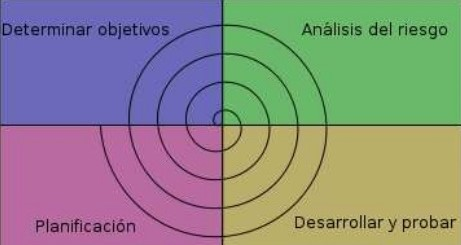
\includegraphics{imgs/metodologia-espiral.jpg}
	\label{fig:Desarrollo en espiral}
\end{figure}

\hspace{1 cm} Se ha mantenido una bit\'acora web en la que se ha ido documentando el progreso en el desarrollo, el cual ha quedado reflejado mediante v\'ideos e im\'agenes en \href{http://jderobot.org/Jvela-tfg}{http://jderobot.org/Jvela-tfg}. Adem\'as el c\'odigo est\'a disponible p\'ublicamente accesible GitHub \href{https://github.com/RoboticsURJC-students/2016-tfg-jorge-vela}{https://github.com/RoboticsURJC-students/2016-tfg-jorge-vela}.


\section{Plan de trabajo}
La planificaci\'on seguida en el desarrollo ha incluido las siguientes fases:

\begin{itemize}
\item{Formaci\'on:} Comprender las distintas herramientas de JdeRobot y trabajar con ellas, creando programas simples y viendo que funcionaban, as\'i como trabajar con distintos robots reales para tener una toma de contacto con ellos y no basarse \'unicamente en un trabajo sobre simulador. 

\item{Desarrollo de la percepci\'on robusta de la baliza:} Comenzar a trabajar con im\'agenes, datos que se obten\'ian y los cambios que pod\'iamos hacer para obtener datos deseados a partir de los cuales mandar \'ordenes. Para \'esto es muy importante el uso de la biblioteca OpenCV.

\item{Desarrollo de control visual de aterrizaje y despegue:} Unir estas dos tecnolog\'ias y conseguir un buen algoritmo que nos permitiera enviar informaci\'on a partir de la imagen de la baliza obtenida en tiempo real a un drone y que \'este la ejecutara de forma correcta y fluida.  

\item{Desarrollo del control de b\'usqueda:} Al igual que en el apartado anterior, hay que enviar informaci\'on al drone en tiempo real diciendo lo que tiene que hacer, pero en este caso diciendo c\'omo se tiene que comportar cuando no hay objetos de inter\'es o cuando hay objetos que posiblemente lo sean. 


\end{itemize}






























